\documentclass{article}
\usepackage[utf8]{inputenc}
\usepackage[a4paper, margin=2.5cm]{geometry}
\usepackage{graphicx}
\usepackage[french]{babel}

\usepackage[default,scale=0.95]{opensans}
\usepackage[T1]{fontenc}
\usepackage{amssymb} %math
\usepackage{amsmath}
\usepackage{amsthm}
\usepackage{systeme}

\usepackage{hyperref}
\hypersetup{
    colorlinks=true,
    linkcolor=blue,
    filecolor=magenta,      
    urlcolor=cyan,
    pdftitle={Overleaf Example},
    }
\urlstyle{same} %\href{url}{Text}

\theoremstyle{plain}% default
\newtheorem{thm}{Théorème}[section]
\newtheorem{lem}[thm]{Lemme}
\newtheorem{prop}[thm]{Proposition}
\newtheorem*{cor}{Corollaire}
%\newtheorem*{KL}{Klein’s Lemma}

\theoremstyle{definition}
\newtheorem{defn}{Définition}[section]
\newtheorem{exmp}{Exemple}[section]
% \newtheorem{xca}[exmp]{Exercise}

\theoremstyle{remark}
\newtheorem*{rem}{Remarque}
\newtheorem*{note}{Note}
%\newtheorem{case}{Case}



\title{Simulation}
\author{Charles Vin}
\date{2021}

\begin{document}
\maketitle

\section{Rappel}
Y'a le word océane si je paume mes feuille. Je vais résumer ici : 
\begin{itemize}
    \item Loi de X : $ P_X(B) = P(X \in B) $ 
    \item Fonction de répartion et ses propriété: $ F_x(t) = P(X \leq t) $  "Avoir la répartion des choses" exemple : quel proportion de la population à un revenu inférieur à t" \begin{itemize}
        \item Croissante 
        \item Caractérise la loi 
        \item Continue à droite avec une limite à gauche en tout point  (cadlag) $ \lim_{x \to a^+} F_X(a) = F_X(a) $ 
        \item Toute fonction cadlag de lim 0 en -inf et 1 en +inf est une fonction de répartion d'une var.
    \end{itemize}
    Exemple dans mon cours papier mdr je sais pas si je le retrouverai le moment venu
    \item Discète == dénombrable = on peut définir une suite
    \item Densité == Fonction de répartion continue
    \item Densité $ F_X (t) = \int_{-\infty }^{t}f_X(x)dx $  \begin{itemize}
        \item N'est pas unique
        \item == dérivé de la fonction de répartion
    \end{itemize}
    \item Quand on cherche $ P(X=x) $ on regarde les sauts de la fonction de répartion sinon c'est toujours égal à 0 comme c'est $ \int_{x}^{x}f_X(y)dy$
    \item 
\end{itemize}
Je reprend tout le cours à fonc à partir d'ici

\section{Simulation par inversion de la fonction de répartion}
\subsection{Cas simple:}
On veux simuler une va X. Sa fonction de répartion est \textbf{continue, strictement croissante}\begin{align*}
    F_X &: R \rightarrow ]0,1[ \\
    &: t \rightarrow F_X(t)
\end{align*}
Comme continue, stric. croissante $\rightarrow$ Bijective (one to one) : $ F_X^{-1} : ]0,1[ $ 
C'est la \textbf{fonction quantile}. Par exemple : 
\[
    F_X^{-1}(\frac{1}{4}) \Leftrightarrow_{Premier quantile} F_X(t) = \frac{1}{4} \Leftrightarrow P(X \leq t) = \frac{1}{4}
.\]
Médiane (quantile à 50 pourcent)
\[
    F_X^{-1}(\frac{1}{2}) \Leftrightarrow P(X \leq t) = \frac{1}{2}
.\]
$F_X^{-1}(\alpha ) $ est le quantile d'ordre $ \alpha  $ de $ X $. \\\\

Que donne la fonction quantile pour un quantile tiré au hasard ? \\
Quelle est la loi de $ F_X^{-1}(U) $ avec $ U \sim Univ(0,1) $ ? Calculons sa fonction de répartion 
\[
    P(F_X^{-1}(U) \leq t) =_{\text{On applique} F_X()} P(U \leq F_X(t))
.\]
\[
    = F_U (F_X(t)) \in [0,1] = F_X(t), \forall t \in R
.\]
$ F_X^{-1} $ et $ X $ ont les mêmes loi car même fonction de répartition
\begin{thm}[]
    Si $ I \sim Unif(]0,1[) $ alors $ F_X^{-1} (U) $ a même loi que X.
\end{thm}

%demander à id pour vérif la fin, en relisant je comprend pas certaine chose

\begin{exmp}[Simulation de la loi de Cauchy (0,1)]
    Soit $ X \sim Cau(0,1) $ de densité $ x \mapsto \frac{1}{\pi (1+x^2)} \text{ sur } \mathbb{R}$ 
    \[
        \forall t \in R, F_X(t) = P(X \leq t) = \int_{-\infty }^{t} \frac{1}{\pi (1+x^2)} dx = \frac{1}{\pi }[\arctan x]^t_{-\infty } = \frac{1}{\pi }(\arctan t - (-\frac{\pi }{2}))  = \frac{\arctan t}{\pi  + \frac{1}{2}}
    .\]
    $ F_X( $ est continue strictement croissante car arctan l'est 
    \[
        \forall \alpha \in ]0,1[, F_X(t) = \alpha \Leftrightarrow \frac{\arctan t}{\pi } + \frac{1}{2} = \alpha \Leftrightarrow \arctan t = \pi (\alpha - \frac{1}{2}) \Leftrightarrow t = tan(\pi (\alpha - \frac{1}{2})) = F_X^-1(\alpha)
    .\]
    Si $ U \sim Unif(]0,1[) $ alors $ \tan (\pi (U-\frac{1}{2})) \sim Cau(0,1)$
    \end{exmp}

    \subsection{Cas Général : fonction de répartition quelconque}
    \begin{defn}[La fonction quantile]
        La \textbf{fonction quantile} de la v.a de $ X $ (aussi appelée pseudo-inverse de la fonction croissante $ F_X $ ) est la fonction :
        \begin{align*}
            F_x^-1 : &]0,1[ \longrightarrow \mathbb{R} \\ 
                    & \alpha \mapsto F_X^-1(\alpha ) = \inf \{t \in R, F_X(t) \geq \alpha \}
        \end{align*} 
        Si $ F_X $ est bijective i.e continue strictement croissante, $ F_X^-1 $ est bien la réciproque de $ F_X $ : 
        \[
            \forall \alpha \in ]0,1[, F_X(F_X^-1(\alpha )) = \alpha 
        .\]
        \[
            \text{et } \forall t \in R, F_X^-1 ( F_X(t)) = t
        .\]
        Si $ F_X $ n'est pas bijective, il y a des $ \alpha  $ et des $ t $ pour lesquels ces inégalités ne sont plus vraies et $ F_X^-1 $ n'est pas la réciproque de $ F_X $, mais la fonction quantile $ F_X^-1 $ reste bien définie sur ]0,1[.
    \end{defn}




    \textbf{Visualisation graphique:} \\\\
    La où $ F_X $ est continue strictement croissante :  
    \begin{figure}[!htbp]
        \centering
        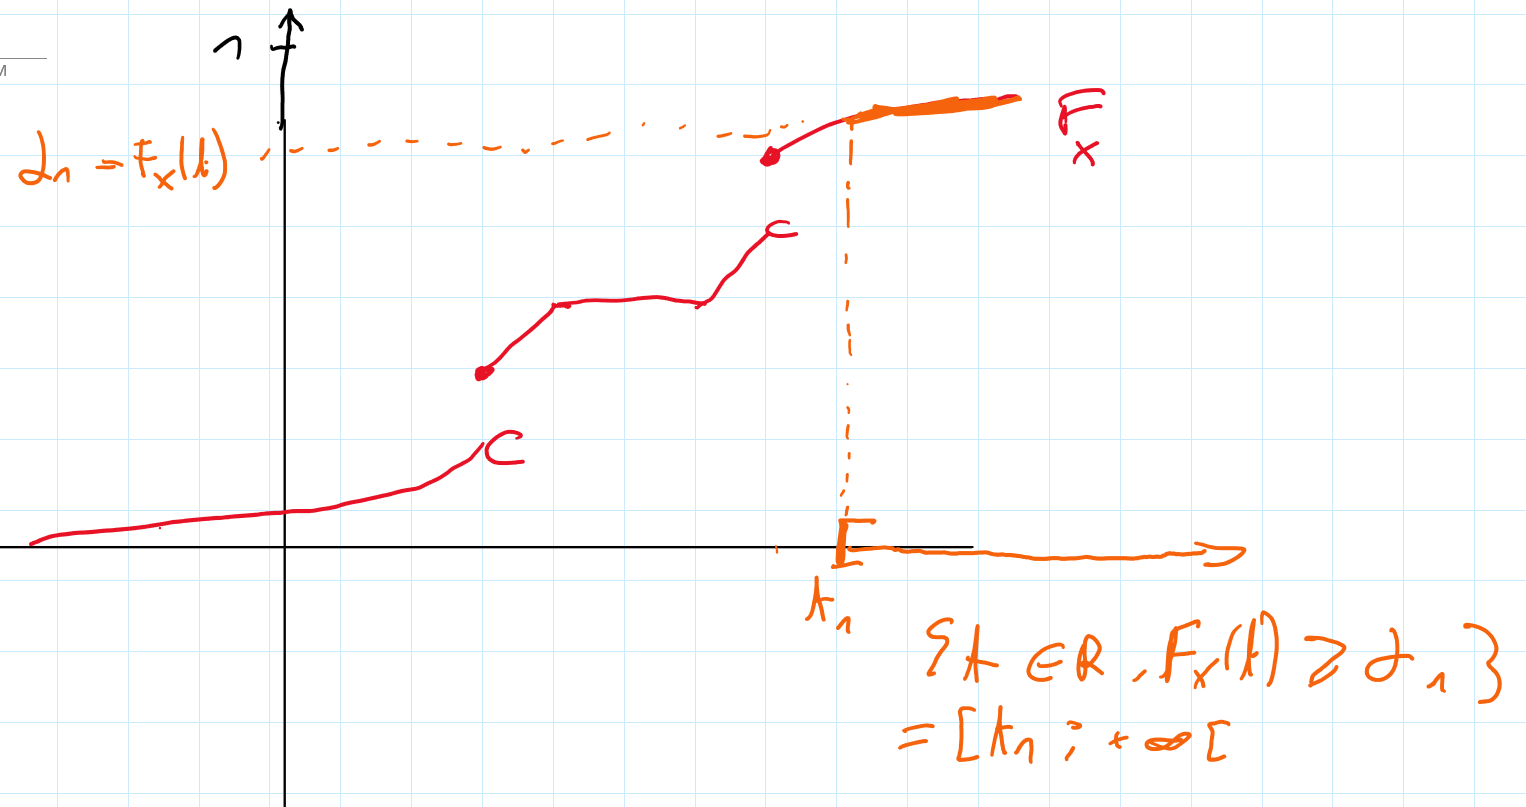
\includegraphics[width=.75\textwidth]{figures/figure1.png}
        \caption{La où $ F_X $ est continue strictement croissante}
        \label{}
    \end{figure}
    
    \[
        F_X^-1(\alpha _1) = inf({t \in R, F_X(t) \geq \alpha _1 }) = inf([t_1 ; +\infty[) = t_1
    .\]
    Ici : $ F_X^1 (F_X(t_1)) = t_1$ et $ F_X(F_X^-1(\alpha _1)) = \alpha 1$  \\\\
    

    Là où $ F_X $ n'est strictement croissante (plateau)
    \begin{figure}[!htbp]
        \centering
        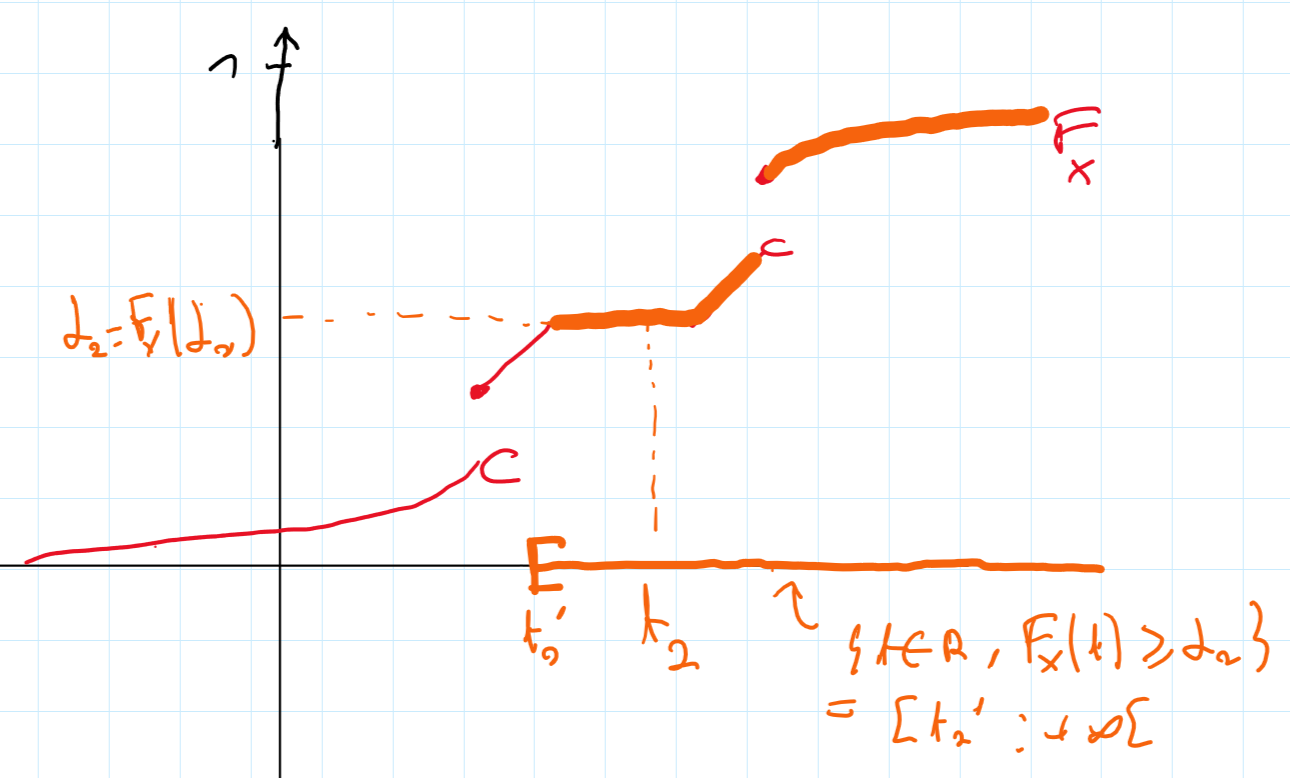
\includegraphics[width=.75\textwidth]{figures/figure2.png}
        \caption{Là où $ F_X $ n'est strictement croissante (plateau)}
        \label{}
    \end{figure}
    \[
        F_X^-1 (\alpha _2) = \inf ({t \in R, F_X(t) \geq \alpha _2}) = t_2' < t_2
    .\]
    Ici : $ F_X^1 (F_X(t_2)) < t_2$ et $ F_X(F_X^-1(\alpha _2)) = \alpha 2$  \\\\


    Là où $ F_X $ est discontinue (saut)
    \begin{figure}[!htbp]
        \centering
        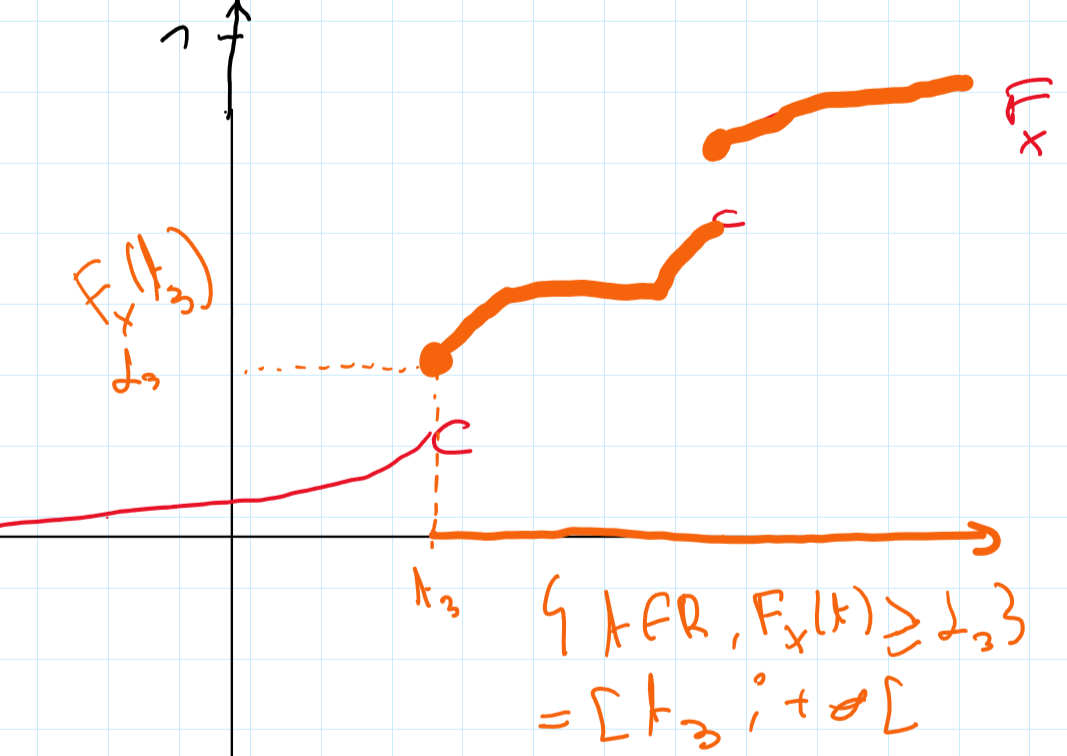
\includegraphics[width=.75\textwidth]{figures/figure3.png}
        \caption{Là où $ F_X $ est discontinue (saut)}
        \label{}
    \end{figure}
    \[
        F_X^-1 (\alpha _3) = \inf ({t \in R, F_X(t) \geq \alpha _3}) = t_3
    .\]
    Ici : $ F_X^1 (F_X(t_3)) < t_3 $ et $ F_X(F_X^-1(\alpha _3)) > \alpha 3$  \\\\
    
    On a toujours 
    \[
        \forall t \in R, F_X^-1(F_X(t)) \leq t 
    .\]
    \[
        \text{et } \forall \alpha \in ]0;1[, F_X(F_X^-1 (\alpha )) \geq \alpha 
    .\]
    Mais ces inégalité peuvent être strictes en certain $ t $ ou $ \alpha  $. \\\\

    La fonction quantile : 
    \begin{figure}[!htbp]
        \centering
        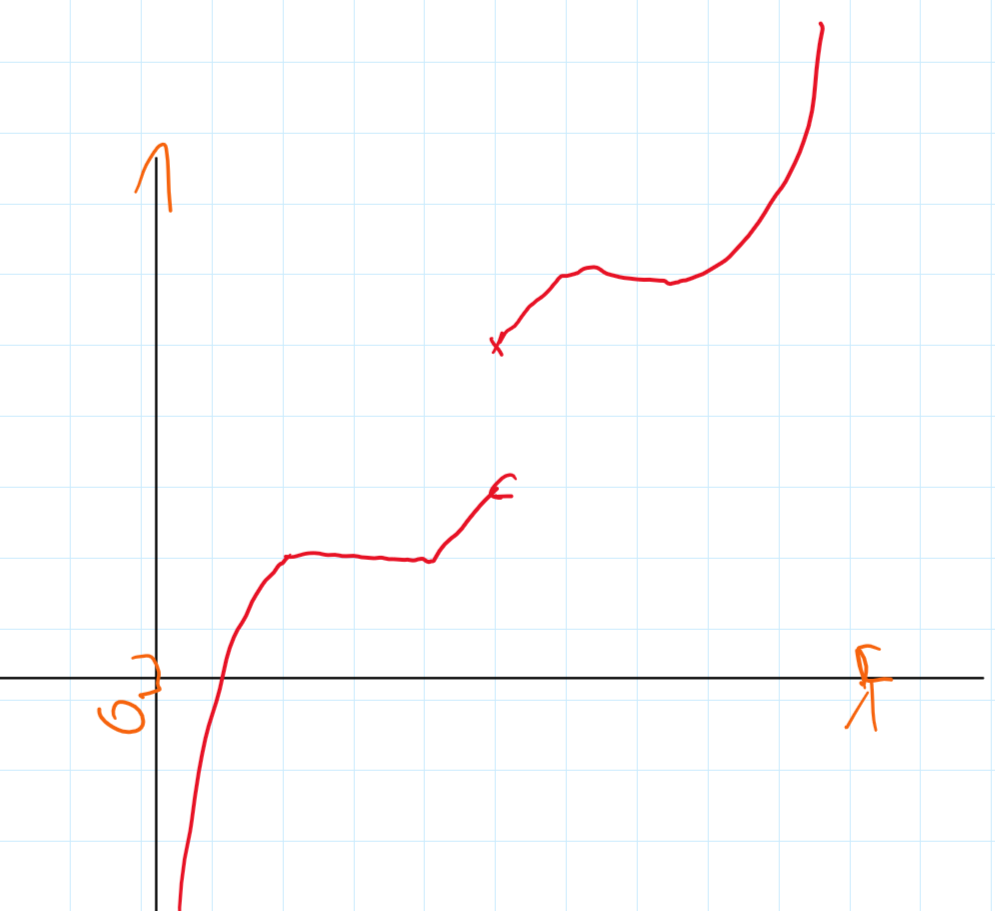
\includegraphics[width=.75\textwidth]{figures/figure4.png}
        \caption{La fonction quantile}
        \label{}
    \end{figure}

    \begin{thm}[]
        Pour toute v.a $ X $ si $ U \sim Unif(]0;1[]) $ alors $ F_X^-1 $ a même loi que $ X $. On simule $ X $ en prenant le quantile d'une valeur choisie au hasard entre 0 et 1. 
        \begin{proof}[Preuve :]
            On a $ F_X^-1(\alpha ) \leq t \Leftrightarrow \leq F_X(t) $ car si $ \alpha \leq F_X(t) $ alors $ t \in \{s \in R, F_X(s) \geq \alpha \} $ donc $ t \geq \inf \{s \in R, F_X(s) \geq \alpha\} = F_X^-1(\alpha )$. La réciproque est vrai aussi (exo). \\ 
            Si $ U \sim Unif(]0,1[) P(F_X^-1(U) \leq t) = P(U \leq F_X (t)) = F_X(t) $ car $ F_X(t) \in [0,1] $ donc $ F_X^-1(U)$ et $X$ ont même fonction de répartition.
        \end{proof}
        
        \begin{exmp}[Simulation des lois exponentielles]
            $ X \sim Exp(\lambda ) $ si \begin{itemize}
                \item $ X $ a pour densité : $ X \mapsto \lambda e^{-\lambda x}\mathbb{1}_{x>0}() $ 
                \item $ X $ a pour fonction de répartition $ (1-e^{- \lambda x}) \mathbb{1}_{x>0}()$ 
            \end{itemize}
            $ F_X $ n'est pas bijective 
            
            \begin{align*}
                \forall \alpha \in ]0;1[, F_X^-1 &= \inf \{t \in R, F_X(t) \geq \alpha \} \\
                        & = \inf \{t \in R^+_*, F_X(t) \geq x\} \\
                        & = \inf \{t \in R^+_*, 1-e^{-\lambda t} \geq x\} \\
                        & = \inf \{t \in R^+_*, t \geq \frac{\ln (1-\alpha  )}{-\lambda } \}  = -\frac{\ln (1-\alpha )}{\lambda }
            \end{align*}
            Si $ U \sim Unif(]0;1[) $ alors $ \frac{-\ln (1-U)}{\lambda } \sim Exp(\lambda ) $ . \\ 
            On vérifie facilement que $ U \sim Unif(]0;1[) \Leftrightarrow 1_U \sim Unif(]0;1[) $ \\ 
            Conclusion : Si 
            \[
                U \sim Unif(]0;1[),  \frac{-\ln (U)}{\lambda } \sim Exp(\lambda )
            .\]
        \end{exmp}

        \begin{exmp}[du temps d'attente de la personne ponctuelle]
            
            \[
                F_X(t) = \systeme*{
                    0 \text{ si } t<0, 
                    \frac{t+5}{20} \text{ si } 0 \leq t \leq 15,
                    1 \text{ si } t \geq 15
                }
            .\]
            Si $ \alpha \in ]0;1/4] $ (on peut prendre le 1/4 ça marche) 
            \[
                F_X^-1 (\alpha ) = \inf \{t \in R, F_X(t) \geq \alpha \} = \inf \{[0; + \infty [\} = 0
            .\]
            Si $ \alpha \in ]1/4 ; 1[ $ :
            \[
                F_X^-1 (\alpha ) = \inf \{t \in R, F_X(t) \geq \alpha \} = \inf \{t \in R, \frac{t+5}{20} \geq \alpha\} = 20 \alpha - 5
            .\]
            Voir graph dans le cours de quelqu'un. \\
            Si $ U \sim Unif(]0,1[) $ 
            \[
                F_X^-1(U) = (20U-5) \mathbb{1}_{U>1/4}() = \max (0,20U-5) \text{ à même loi que } X
            .\]
            
        \end{exmp}
    \end{thm}
\end{document}